% Chapter Template

\chapter{Dataset} % Main chapter title

\label{ch:04} % Change X to a consecutive number; for referencing this chapter elsewhere, use \ref{ChapterX}

%----------------------------------------------------------------------------------------
%	SECTION 1
%----------------------------------------------------------------------------------------

\section{Synthetic Dataset}
To train a deep learning model with supervised learning scheme, a dataset should require two principles, truth-worthy ground-truth and comprehensive scenarios. The depth map captured by Kinect is not satisfied the first requirement since it is usually semi-dense with a number of missing pixels, as shown in Figure \ref{fig:kinect-depth}. Therefore, a more elaborate depth map is required for the training work. In this thesis, a dataset called ``synthetic50-5" is created for the training works.


\subsection{Resource}
\cite{data1}, \cite{data2}, \cite{data3} and \cite{data4} published a set of point cloud dataset on the internet for computer vision task research. These point clouds are scanned from real objects using high resolution scanners like Cyberware 3030 MS+ and calibrated with post processing. Each objects has been scanned for hundreds of times for an exhaustive completion for the origin objects, which is up to millions points. (\cite{data1}). The dense point clouds makes the normal inference task trivial since the neighbor based method performs good enough for these kind of task. Some of the point cloud even equipped with pre-computed normal map based on more advanced methods. They all provides the accurate ground-truth for the supervised learning method.

The ``synthetic50-5", is a datset with 50 point clouds as training set and 5 point clouds as test set. The dataset is created base on the work of this thesis and using for normal inference task. Figure \ref{fig:dataset-demo} gives the illustrations of some objects. Appendix \ref{AppendixA} gives a full version of dataset models.

\begin{figure}[!h]
	\centering
	\begin{subfigure}[b]{0.23\linewidth}
		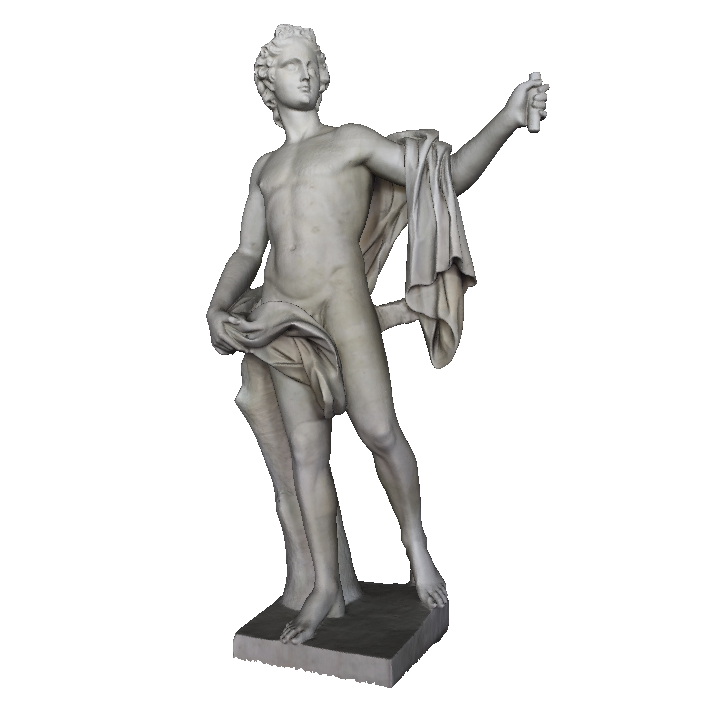
\includegraphics[width=\linewidth]{./Figures/train-dataset/00.apoll.png}
		\caption{apoll}
	\end{subfigure}
	\begin{subfigure}[b]{0.23\linewidth}
		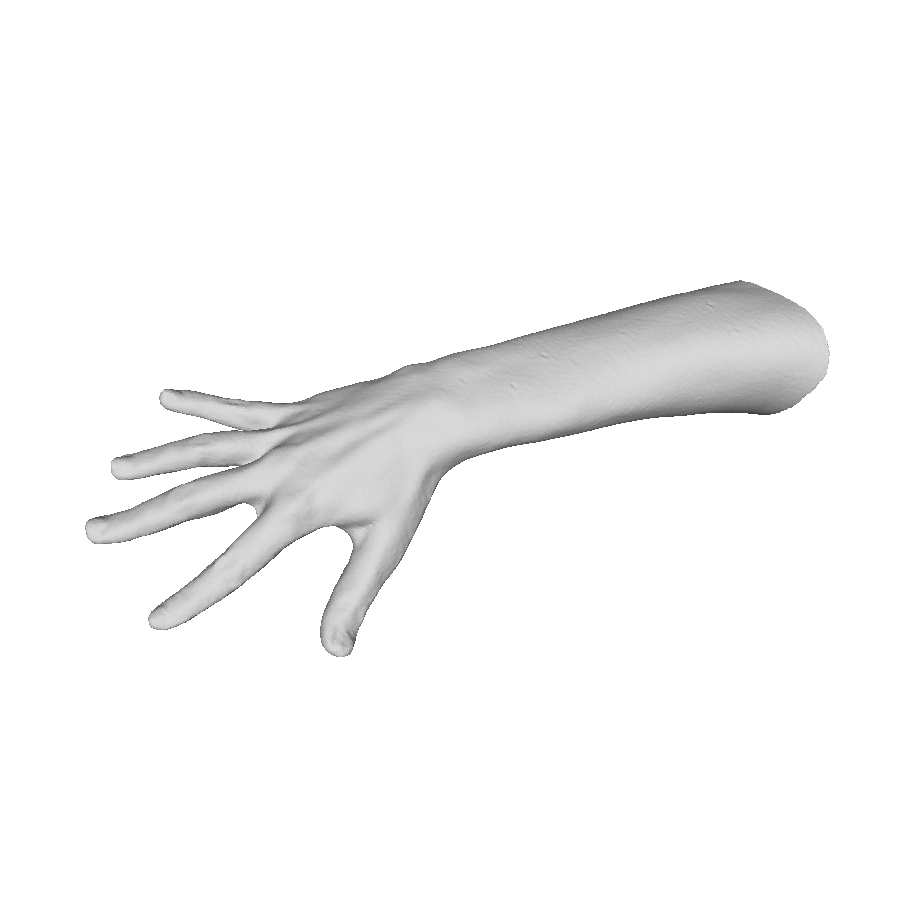
\includegraphics[width=\linewidth]{./Figures/train-dataset/01.arm.png}
		\caption{arm}
	\end{subfigure}
	\begin{subfigure}[b]{0.23\linewidth}
		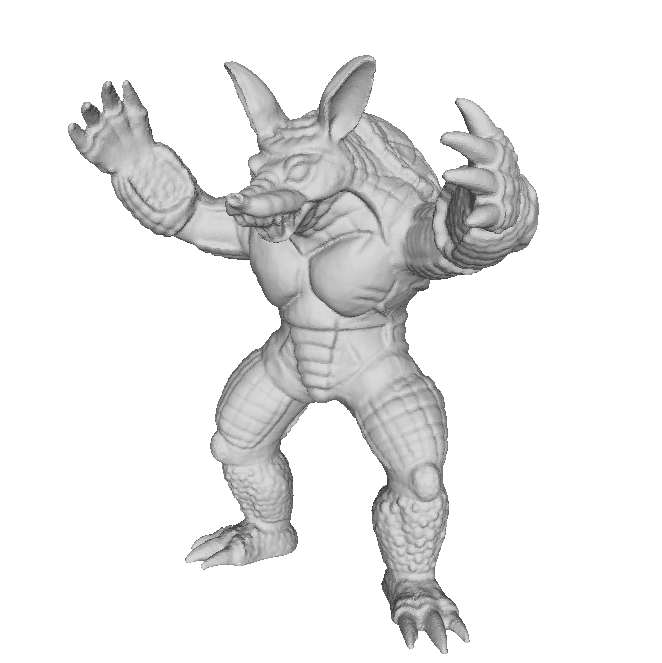
\includegraphics[width=\linewidth]{./Figures/train-dataset/02.armadillo.png}
		\caption{armadillo}
	\end{subfigure}
	\begin{subfigure}[b]{0.23\linewidth}
		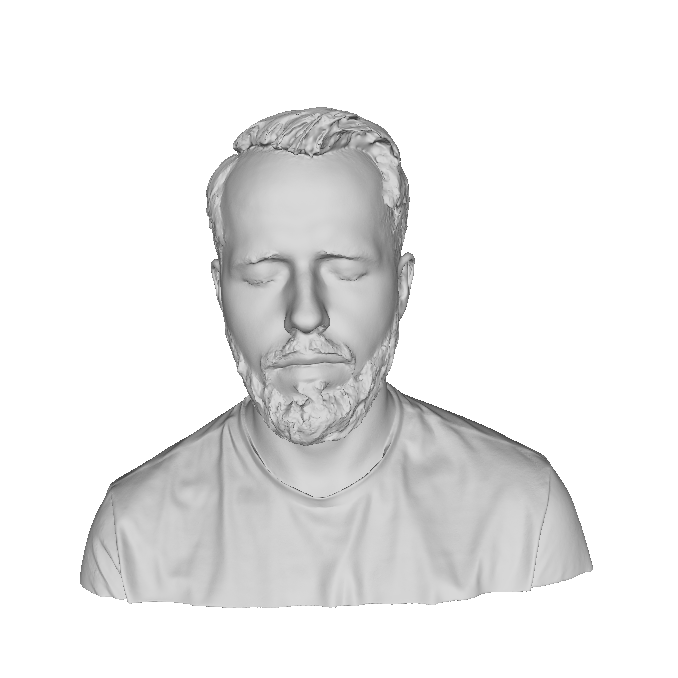
\includegraphics[width=\linewidth]{./Figures/train-dataset/03.bearded-guy.png}
		\caption{bearded-guy}
	\end{subfigure}
	
	\begin{subfigure}[b]{0.23\linewidth}
		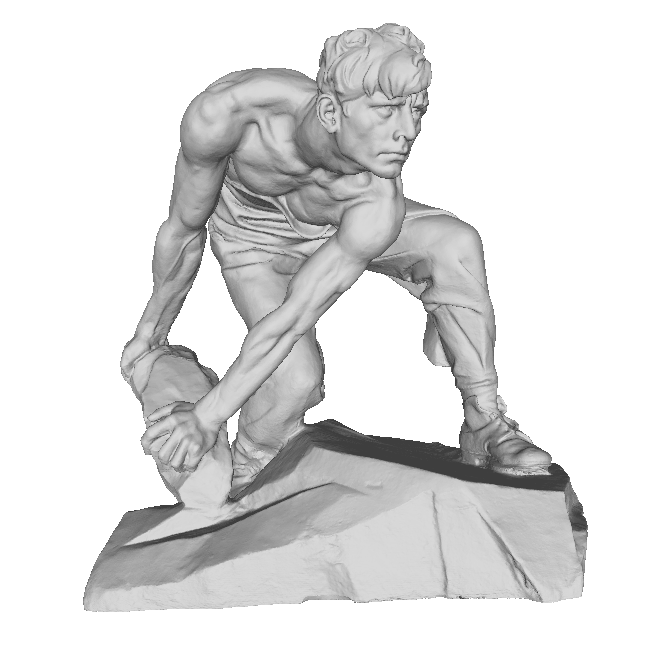
\includegraphics[width=\linewidth]{./Figures/train-dataset/04.bronze-sculpture.png}
		\caption{bronze-sculpture}
	\end{subfigure}
	\begin{subfigure}[b]{0.23\linewidth}
		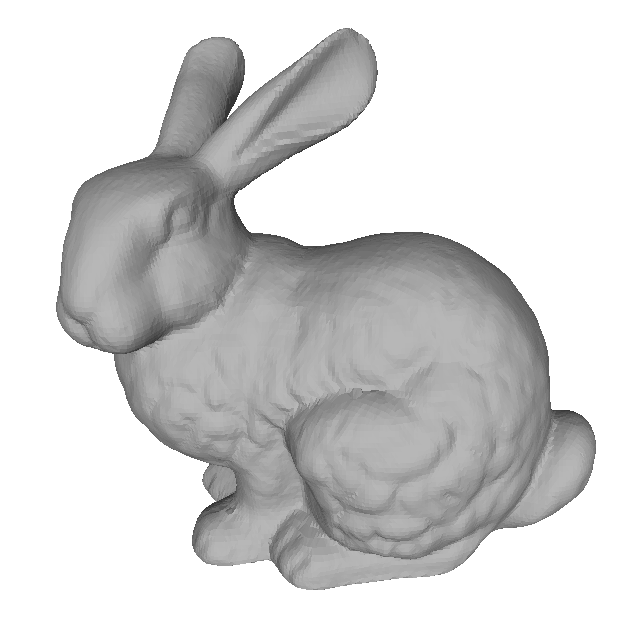
\includegraphics[width=\linewidth]{./Figures/train-dataset/05.bunny.png}
		\caption{bunny}
	\end{subfigure}
	\begin{subfigure}[b]{0.23\linewidth}
		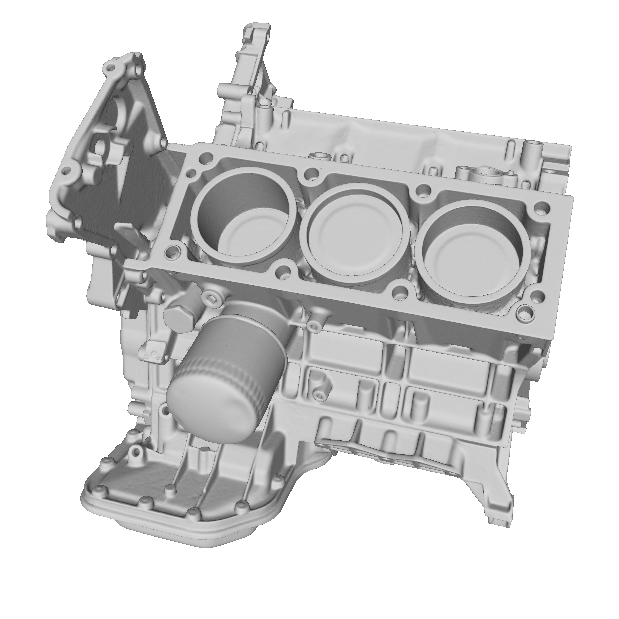
\includegraphics[width=\linewidth]{./Figures/train-dataset/06.car-engine.png}
		\caption{car-engine}
	\end{subfigure}
	\begin{subfigure}[b]{0.23\linewidth}
		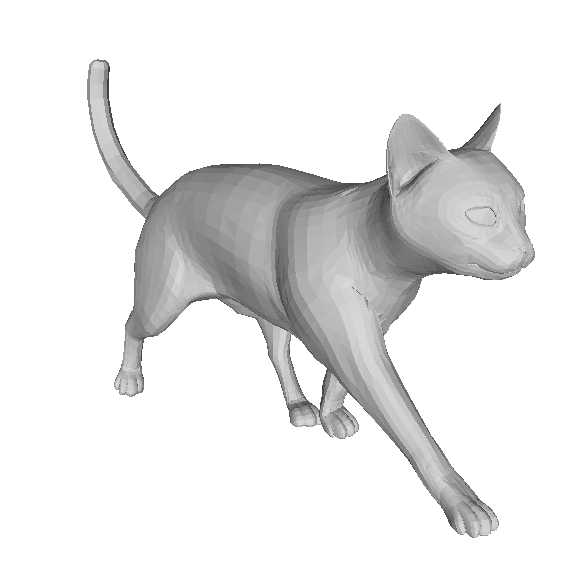
\includegraphics[width=\linewidth]{./Figures/train-dataset/07.cat.png}
		\caption{cat}
	\end{subfigure}
	
	\label{fig:dataset-demo}
	\caption{Point clouds scanned by high resolution scanners}
\end{figure}


\subsection{Synthesize Scenes using Unity}
In order to fit the using scenario of Kinect as much as possible, the dataset consists of the generated synthetic 3D scenes via Unity, which is a game engine using for 3D games creation. 

In the synthetic scenes from engine, the object is placed on a cylinder platform, which is lighted by a directional light nearby. A camera focus on the platform and captured the scene. The layout in the game engine is shown in Figure \ref{fig:unity-workplace}. In order to simulate more scenarios, the positions of the camera and directional light are randomly changed in each new scene. For 50 training objects, 1000 scenes are generated and each scene is saved in 3 kinds of resolutions $ 512\times512\times3 $, $ 256\times256\times3 $ and $ 128\times128\times3 $.

\begin{figure}[h!]
	\centering
	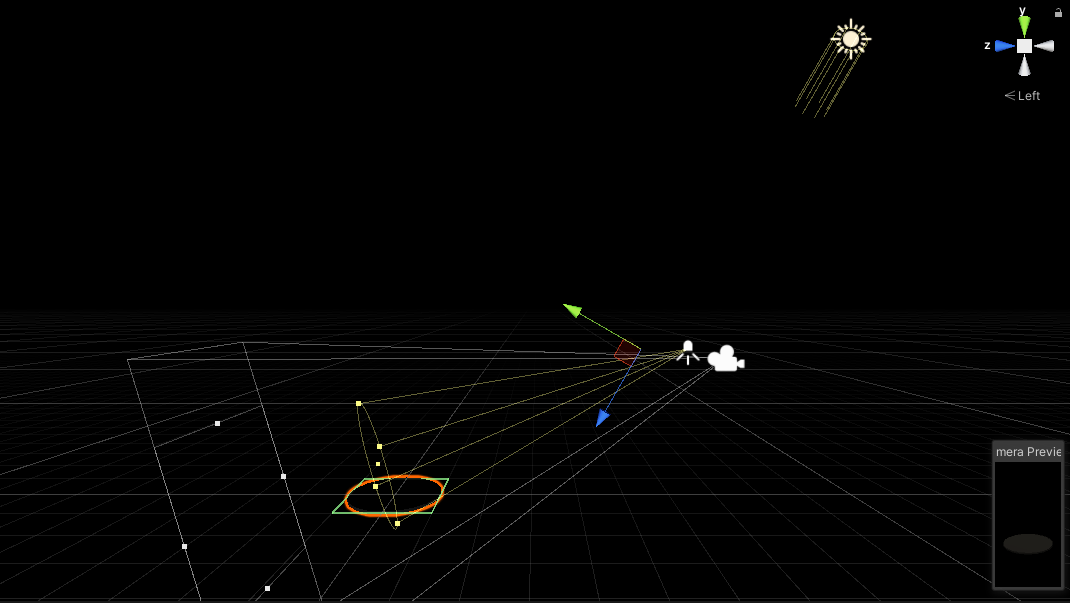
\includegraphics[width=.8\textwidth]{./Figures/unity-workplace.PNG}
	\caption{The layout of synthetic scenes generation in Unity.}
	\label{fig:unity-workplace}
\end{figure}

The main advantage using generated scene is the availability of complete information. The depth map can be captured in a loss-free way. The corresponding normal map can also be safely considered as ground truth. And the scale of the dataset is easy to control.

For each scene, following information is recorded
\begin{table}
	\caption{The information saved for each scene in ``synthetic50-5".}
	\label{tab:data-files}
	\centering
	\begin{tabular}{l l}
		\toprule
		\tabhead{Data} & \tabhead{Size} \\
		\midrule
		Depth map & $ 512\times512\times3 $ \\
		\hline 
		Depth range  & $ 2\times1 $ \\  
		\hline
		Grayscale Image	& $ 512\times512\times1 $ \\  
		\hline 
		Normal Map &  $ 512\times512\times3 $  \\
		\hline 
		Light Position &  $ 3\times1 $  \\
		\hline
		Camera Intrinsic Matrix &  $ 3\times 3 $  \\
		\hline 
		Camera Extrinsic Matrix &  $ 3\times 4 $  \\
		\hline 
		\bottomrule\\
	\end{tabular}
\end{table}

A depth map $ D $ is captured by a depth camera in Unity, which is a 1 channel image that contains the information relating to the distance of the surfaces of the scene objects from a viewpoint. It can be saved as a 16-bit grayscale image, i.e. each pixel in range $0 - 65535$. The grayscale image can be used as guided normal inference task and also as a readable scene for human. The gray-color is converted from RGB color based on following equation 
\[ gray: \frac{r+2g+b}{4}  \]
The normal map is the tangent surface normal, which is saved in 32-bit RGB color image. The surface normal and its corresponding RGB color can be converted based on following equation:
\[  \]
If consider the relation between Lambertian reflection and normal direction, the light source can be used to calculate the reflect direction of each point.
The camera intrinsic and extrinsic matrix helps point cloud calculation.

It is necessary to point out again that ``synthetic50-5" aiming to rebuild the using scenarios of Kinect, where all types of the generated data files shown in Table \ref{tab:data-files} are also the same format of the Kinect data.





\subsection{Convert to Point Cloud}
\label{sec:depth-map-to-point-cloud}
The depth map can be converted to 3D vertex point cloud as the input of the normal inference model. 




\subsection{Point Cloud calculation}

Consider a 3-dimensional Euclidean space. Use $ z $ axis denotes the depth. The $ x  $ and $ y $ axes perpendicular with each other. For a pixel $ (u,v) $ on depth map, its value $ D(u,v) $ is the $ Z $ component of the 3D point $P_C = (X,Y,Z) $ corresponding the camera origin. Based on the triangle similarity, we can get other two components $ X $ and $ Y $ as follows

\begin{dgroup*}
	
	\begin{dmath*}
		X = \frac{uZ}{fk_u}
	\end{dmath*}
	\begin{dmath*}
		Y = \frac{vZ}{fk_v}
	\end{dmath*}
\end{dgroup*}

where $ fk_u, fk_v $ is the focal length in pixels align $ u $ and $ v $ axes.
It can be further converted to world coordinate system based on extrinsic matrix $ R $ and $ t $, that is
\[P_W = P_CR+t \]

\subsection{Point Cloud Normalization}


\label{sec:dataset-normalization}
%% How to represent input tensor, to make it fast converse

The vertices have been normalized before feed them into the model. The depth range of each scene is shown in Figure \ref{fig:data-range}.
The sizes of each training object are various, whereas it should be as an invariant value for the training model. Thus the normalization is required before feed training objects into the models. Figure \ref{fig:data-range} shows the fluctuation of extreme values and their ranges in 100 random training items. Table \ref{tab:data-range} gives the corresponding average values.
%\begin{figure}[!h]
%	\centering
%	{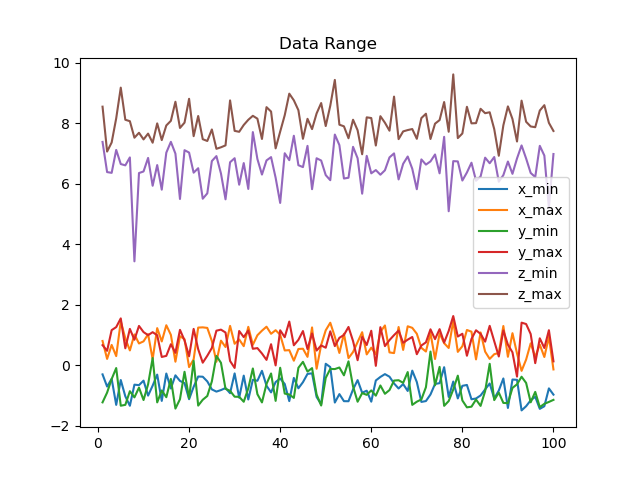
\includegraphics[width=0.45\textwidth]{./pic/Data_Extreme.png}}
%	{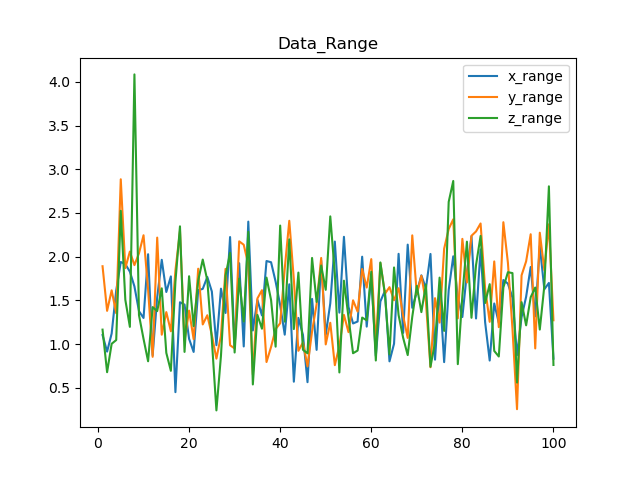
\includegraphics[width=0.45\textwidth]{./pic/Data_Range.png}}
%	\label{fig:data_range}
%	\caption{Left: Extreme value in 3 axis; Right: Vertex range in 3 axis}
%\end{figure}

\begin{table}[!h]
	\centering
	\begin{tabular}{|c|c|c|c|}
		\hline
		Axis & Range & Min & Max\\
		\hline
		X & 1.48 & -0.75 & 0.73\\
		Y & 1.56 & -0.76 & 0.80\\
		Z & 1.47 & 6.53 & 8.00\\
		\hline
	\end{tabular}
	\caption{The ranges and extreme values of each axis. The extreme min and max values of both X axis and Y axis are close to $ -0.75 $ and $ 0.75 $ separately. The case for Z axis is $ 6.5 $ and $ 8.0 $ separately. However, the range of three axes are relatively similar, around 1.5. 
	}
	\label{tab:data-range}
\end{table}


For the normalization, first we translate the point to the original point as much as possible, then choose the range value of one axis as a scale factor, normalize it to a unit object. 

\begin{equation}\label{eq:normalization}
	U^a = (V^a - V^a_{min}) / s  \quad  \text{for } a \text{ in }  X,Y,Z \text{ axis}
\end{equation}
where $ V^a_{min} $ denote the minimum value appeared in axis $ a $, $ s $ is the range of an axis, which can be any one of X, Y, or Z axis. 

In this thesis, the range of X is chosen as scale factor for each scene.



As discussed in \ref{sec:dataset-normalization}, the 3D vertex point cloud should be moved to origin point and normalize in range $ [0,1] $ to acquire a scale invariant feature.


\begin{dgroup*}
	
	\begin{dmath*}
		X_n =\frac{X-\min(X)}{s}
	\end{dmath*}
	\begin{dmath*}
		Y_n = \frac{Y-\min(Y)}{s}
	\end{dmath*}
	
	\begin{dmath*}
		Z_n = \frac{Z-\min(Z)}{s}
	\end{dmath*}
	
	
\end{dgroup*}

where $ s $ is a scale factor, 

\begin{dmath*}
	s = \max(X)-\min(X)
\end{dmath*}
It is calculated as the range in $ X $ axis, but theoretically can be used by $ Y $ or $ Z $ axes as well.




\subsection{Noise}
\label{sec:noise}
The raw depth maps captured by Kinect usually have missing pixels. As shown in Figure \ref{fig:depth_map_kinect}.
Observing the depth map, the missing pixels distributed all around the scene. Therefore an uniformly distributed pixel-delete noise is used for noise simulation. 
It is reasonable that the noise intensities in different scenes are various. Some scenes have more missing pixels and some have less. It enables the model to not only learn scenarios with noise, but also with small minority noise or even without noise. In the noised dataset, the noise intensity is a x-percent pixel dropoff operation. For example, noise-intensity-10 means removes 10\% pixels.
Figure \ref{fig:noise-intensity} shows the visualization of depth map after adding noise.
%% add noise image
\begin{figure}[!h]
	\centering
	{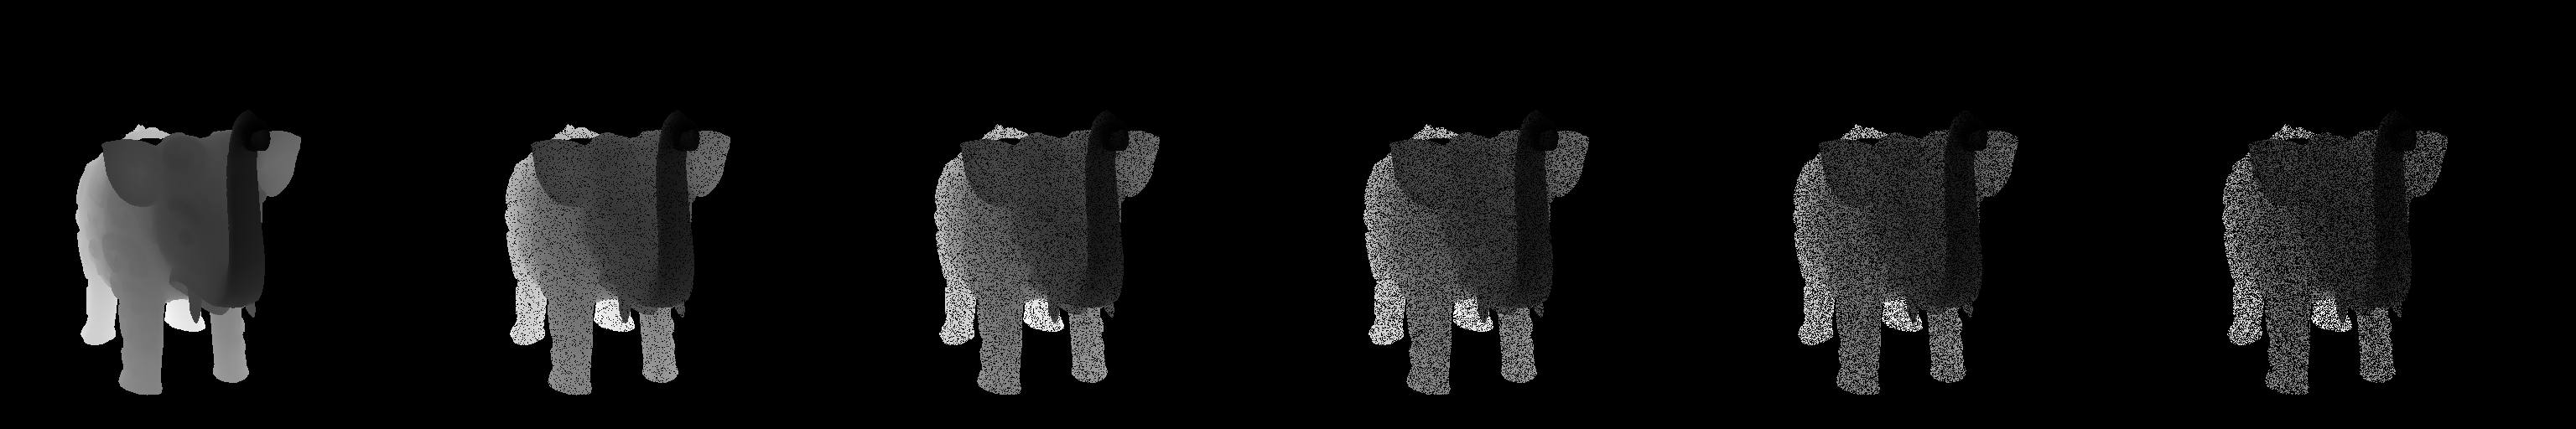
\includegraphics[width=.9\textwidth]{./Figures/add_noise_depth.png}}
	\decoRule	
	\caption{Noise-intensity on 0, 10, 20, 30, 40, 50. Object Name: elephant-zun-lid.}
	\label{fig:noise-intensity}
\end{figure}


\subsection{Fit to PyTorch}
In order to saving the training time, the dataset is compressed in PyTorch format. The structure of a single item is shown in Table \ref{tab:tensor-structure}.
\begin{table}
	\caption{The structure of a single tensor in the dataset.}
	\label{tab:tensor-structure}
	\centering
	\begin{tabular}{l l}
		\toprule
		\tabhead{Name} & \tabhead{Description} \\
		\midrule
		\multirow{3}{*}{input-tensor}  & Vertex \\  & Image \\  & Light Direction \\
		\hline
		\multirow{4}{*}{output-tensor}  & GT-Normal  \\ & GT-Normal * GT-Light-Direction \\ & Image \\ & GT-Light-Direction \\
		\hline
		Light position & light position \\
		\hline 
		\multirow{3}{*}{Camera Matrix}  & K \\  & R \\  & t \\
		\hline 
		\multirow{2}{*}{Depth Range}  & minDepth \\  & maxDepth \\
		\hline
		\bottomrule\\
	\end{tabular}
\end{table}




\section{Real Dataset}

The real dataset is the depth map and rgb image captured via Kinect...


\section{Metrics for evaluation}
Angle Loss

